\documentclass{report}
\usepackage{comment}
\usepackage{fancyhdr}
\pagestyle{fancy}

\rhead{ \thepage}
\cfoot{  }
\rfoot{Suryanshu, 22BCE0820}
\renewcommand{\headrulewidth}{0.4pt}
\renewcommand{\footrulewidth}{0.4pt}
\usepackage{listings}
\title{\textbf{Finlatics \\ Programme: Business Analytics \\ Project 1}}

\author{Suryanshu}
\usepackage{titlesec}
\titleformat
{\chapter} % command
[display] % shape
{\bfseries\Large\itshape} % format
{Business Analytics} % label
{0.5ex} % sep
{
    \rule{\textwidth}{1pt}
    \vspace{1ex}
    \centering
} % before-code
[
\vspace{-0.5ex}%
\rule{\textwidth}{0.3pt}
] % after-code

\usepackage{tikz}
\usetikzlibrary{shapes.geometric, arrows}

\tikzstyle{startstop} = [rectangle, rounded corners, minimum width=3cm, minimum height=1cm,text centered, draw=black, fill=red!30]

%\tikzstyle{process} = [rectangle, minimum width=3cm, minimum height=1cm, text centered, draw=black, fill=orange!30]

\tikzstyle{io} = [trapezium, trapezium left angle=70, trapezium right angle=110, minimum width=1cm, minimum height=1cm, text centered, text width=1.5cm, draw=black, fill=blue!30]

\tikzstyle{layer2} = [rectangle, minimum width=2cm, inner sep=7pt, text centered,  draw=black, fill=orange!30]
\tikzstyle{layer3} = [rectangle, text centered, text width=2.5cm, inner sep=7pt, draw=black, fill=blue!30]
\tikzstyle{layer4} = [rectangle, text centered, text width=2.5cm, inner sep=7pt, draw=black, fill=green!30]

\tikzstyle{decision} = [diamond, minimum width=3cm, minimum height=1cm, text centered, draw=black, fill=green!30]
\tikzstyle{line} = [draw, -latex']
\tikzstyle{arrow} = [thick,->,>=stealth]
\begin{document}
\maketitle
\tableofcontents

\chapter{Project 1 }
\section{Identifying the Root Problem}
The root problem for the company seems to be \emph{``finding it difficult to be at par with its competitors on a year-on-year margin improvement rate which is 11\% v/s 26\% by other comparable IT companies in India.''}

What this implies is that the rate of \emph{rate of profit} the company acrues is less than half at which the industry in general does. To overcome this, there are usually three ways- 
\begin{enumerate}
    \item by lengthening the workday through overtime, thereby increasing the total profit absolutely; 
    \item by increasing the productivity of the worker, thereby increasing the total profit relatively;
    \item by decreasing variable capital whilst mainting the size of the workforce, and hence reducing the total capital invested but increasing the rate of surplus value.
\end{enumerate}
This leaves the company with two options,
\begin{enumerate}
    \item increase the productivity in the sectors in which it already engages in.
    \item increase investment in the sectors which have a tendency to generate a \emph{good margin}.
\end{enumerate}
\newpage
\section{MECE of the Root Problem}
    \begin{figure}[h!]
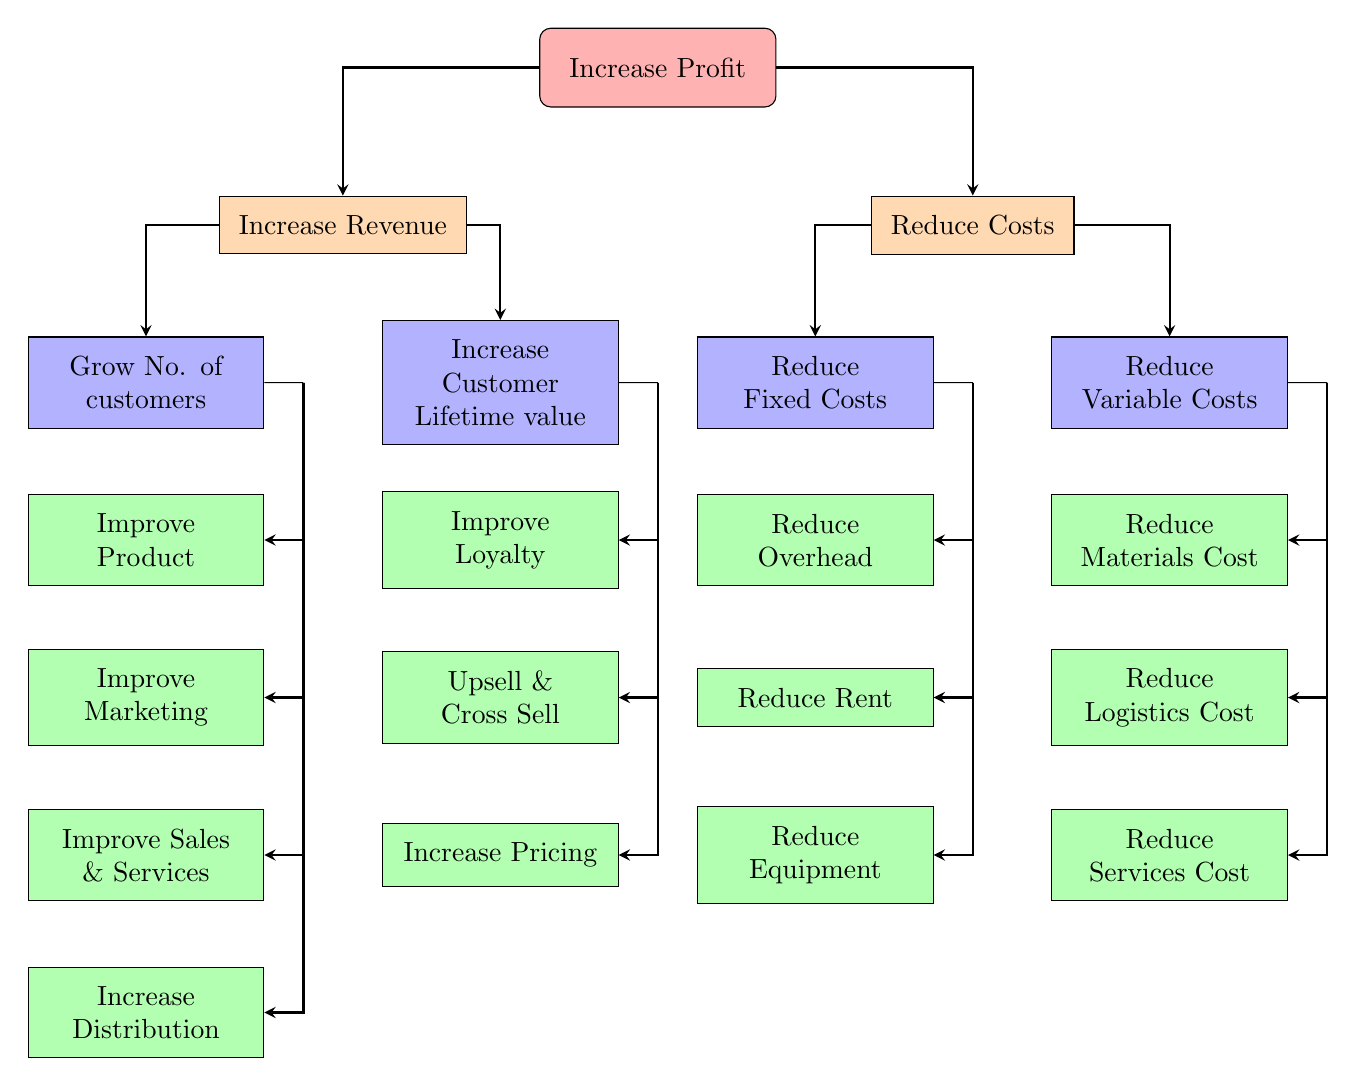
\begin{tikzpicture}[node distance=2cm]
    \node (title) [startstop, xshift=-1cm] {Increase Profit};

    \node (l-layer2) [layer2, below of=title, xshift=-4cm] {Increase Revenue};
    \node (r-layer2) [layer2, below of=title, xshift=4cm] {Reduce Costs};

    \node (ll-layer3) [layer3, below of=l-layer2, xshift=-2.5cm] {Grow No. of customers};
    \node (lr-layer3) [layer3, below of=l-layer2, xshift=2cm] {Increase Customer Lifetime value};
    \node (rl-layer3) [layer3, below of=r-layer2, xshift=-2cm] {Reduce Fixed Costs};
    \node (rr-layer3) [layer3, below of=r-layer2, xshift=2.5cm] {Reduce Variable Costs};

    \node (ll1-layer4) [layer4, below of=ll-layer3] {Improve Product};
    \node (ll2-layer4) [layer4, below of=ll1-layer4] {Improve Marketing};
    \node (ll3-layer4) [layer4, below of=ll2-layer4] {Improve Sales \& Services};
    \node (ll4-layer4) [layer4, below of=ll3-layer4] {Increase Distribution};

    \node (lr1-layer4) [layer4, below of=lr-layer3] {Improve Loyalty};
    \node (lr2-layer4) [layer4, below of=lr1-layer4] {Upsell \& Cross Sell};
    \node (lr3-layer4) [layer4, below of=lr2-layer4] {Increase Pricing};

    \node (rl1-layer4) [layer4, below of=rl-layer3] {Reduce Overhead};
    \node (rl2-layer4) [layer4, below of=rl1-layer4] {Reduce Rent};
    \node (rl3-layer4) [layer4, below of=rl2-layer4] {Reduce Equipment};

    \node (rr1-layer4) [layer4, below of=rr-layer3] {Reduce Materials Cost};
    \node (rr2-layer4) [layer4, below of=rr1-layer4] {Reduce Logistics Cost};
    \node (rr3-layer4) [layer4, below of=rr2-layer4] {Reduce Services Cost};
    
    \draw [arrow] (title) -| (l-layer2);
    \draw [arrow] (title) -| (r-layer2);

    \draw [arrow] (l-layer2) -| (ll-layer3);
    \draw [arrow] (l-layer2) -| (lr-layer3);

    \draw [arrow] (r-layer2) -| (rl-layer3);
    \draw [arrow] (r-layer2) -| (rr-layer3);

    \draw (ll-layer3) -- (-5.5, -4.0);
    \draw (lr-layer3) -- (-1, -4.0);
    \draw (rl-layer3) -- (3.0, -4.0);
    \draw (rr-layer3) -- (7.5, -4.0);

    \draw [arrow] (-5.5, -4.0) |- (ll1-layer4);
    \draw [arrow] (-5.5, -4.0) |- (ll2-layer4);
    \draw [arrow] (-5.5, -4.0) |- (ll3-layer4);
    \draw [arrow] (-5.5, -4.0) |- (ll4-layer4);

    \draw [arrow] (-1, -4.0) |- (lr1-layer4);
    \draw [arrow] (-1, -4.0) |- (lr2-layer4);
    \draw [arrow] (-1, -4.0) |- (lr3-layer4);

    \draw [arrow] (3.0, -4.0) |- (rl1-layer4);
    \draw [arrow] (3.0, -4.0) |- (rl2-layer4);
    \draw [arrow] (3.0, -4.0) |- (rl3-layer4);

    \draw [arrow] (7.5, -4.0) |- (rr1-layer4);
    \draw [arrow] (7.5, -4.0) |- (rr2-layer4);
    \draw [arrow] (7.5, -4.0) |- (rr3-layer4);
\end{tikzpicture}
        \caption{\emph{Obtained through Notes}}
    \end{figure}
\newpage
\section{Profitability Tree}
    \begin{figure}[h!]
        \centering
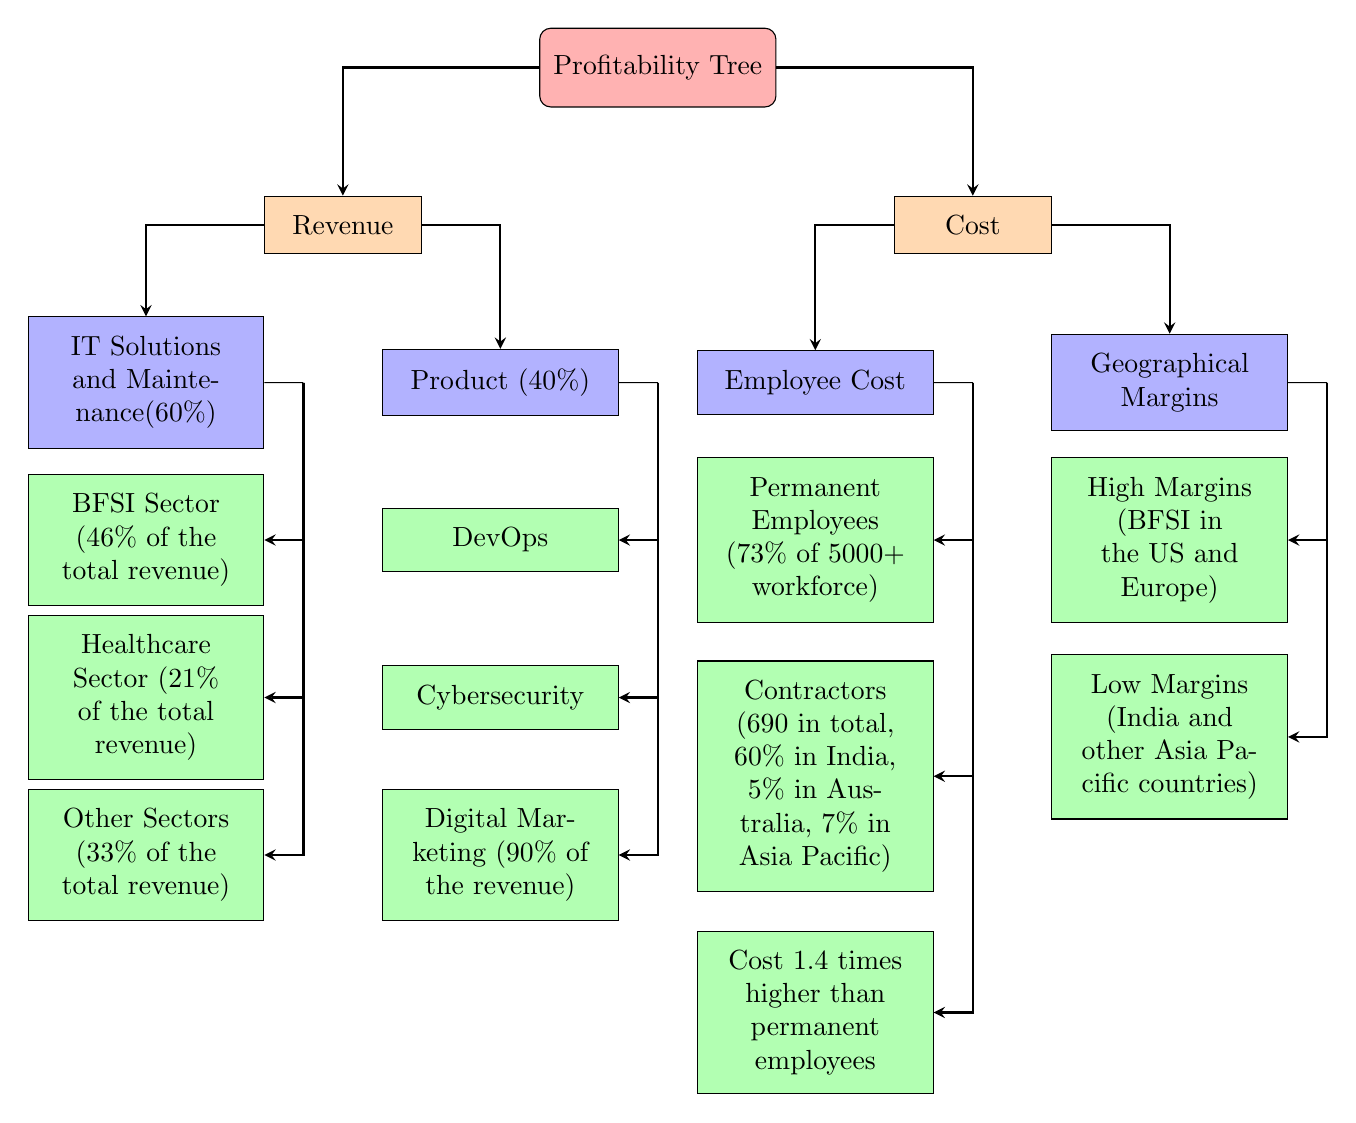
\begin{tikzpicture}[node distance=2cm]
    \node (title) [startstop, xshift=-1cm] {Profitability Tree};

    \node (l-layer2) [layer2, below of=title, xshift=-4cm] {Revenue};
    \node (r-layer2) [layer2, below of=title, xshift=4cm] {Cost};

    \node (ll-layer3) [layer3, below of=l-layer2, xshift=-2.5cm] {IT Solutions and Maintenance(60\%)};
    \node (lr-layer3) [layer3, below of=l-layer2, xshift=2cm] {Product (40\%)};
    \node (rl-layer3) [layer3, below of=r-layer2, xshift=-2cm] {Employee Cost};
    \node (rr-layer3) [layer3, below of=r-layer2, xshift=2.5cm] {Geographical Margins};

    \node (ll1-layer4) [layer4, below of=ll-layer3] {BFSI Sector (46\% of the total revenue)};
    \node (ll2-layer4) [layer4, below of=ll1-layer4] {Healthcare Sector (21\% of the total revenue)};
    \node (ll3-layer4) [layer4, below of=ll2-layer4] {Other Sectors (33\% of the total revenue)};

    \node (lr1-layer4) [layer4, below of=lr-layer3] {DevOps};
    \node (lr2-layer4) [layer4, below of=lr1-layer4] {Cybersecurity};
    \node (lr3-layer4) [layer4, below of=lr2-layer4] {Digital Marketing (90\% of the revenue)};

    \node (rl1-layer4) [layer4, below of=rl-layer3] {Permanent Employees (73\% of 5000+ workforce)};
    \node (rl2-layer4) [layer4, below of=rl1-layer4, yshift=-1cm] {Contractors (690 in total, 60\% in India, 5\% in Australia, 7\% in Asia Pacific)};
    \node (rl3-layer4) [layer4, below of=rl2-layer4, yshift=-1cm] {Cost 1.4 times higher than permanent employees};

    \node (rr1-layer4) [layer4, below of=rr-layer3] {High Margins (BFSI in the US and Europe)};
    \node (rr2-layer4) [layer4, below of=rr1-layer4, yshift=-0.5cm] {Low Margins (India and other Asia Pacific countries)};
    
    \draw [arrow] (title) -| (l-layer2);
    \draw [arrow] (title) -| (r-layer2);

    \draw [arrow] (l-layer2) -| (ll-layer3);
    \draw [arrow] (l-layer2) -| (lr-layer3);

    \draw [arrow] (r-layer2) -| (rl-layer3);
    \draw [arrow] (r-layer2) -| (rr-layer3);

    \draw (ll-layer3) -- (-5.5, -4.0);
    \draw (lr-layer3) -- (-1, -4.0);
    \draw (rl-layer3) -- (3.0, -4.0);
    \draw (rr-layer3) -- (7.5, -4.0);

    \draw [arrow] (-5.5, -4.0) |- (ll1-layer4);
    \draw [arrow] (-5.5, -4.0) |- (ll2-layer4);
    \draw [arrow] (-5.5, -4.0) |- (ll3-layer4);

    \draw [arrow] (-1, -4.0) |- (lr1-layer4);
    \draw [arrow] (-1, -4.0) |- (lr2-layer4);
    \draw [arrow] (-1, -4.0) |- (lr3-layer4);

    \draw [arrow] (3.0, -4.0) |- (rl1-layer4);
    \draw [arrow] (3.0, -4.0) |- (rl2-layer4);
    \draw [arrow] (3.0, -4.0) |- (rl3-layer4);

    \draw [arrow] (7.5, -4.0) |- (rr1-layer4);
    \draw [arrow] (7.5, -4.0) |- (rr2-layer4);
\end{tikzpicture}
        \caption{\emph{Given in the Problem Statement}}
    \end{figure}
    \newpage
\section{Potential Growth in Different Sectors and Geographical Locations:}

\subsection{India}
Though the profit margins in business in India (9\%) are quite low, \textbf{BFSI} and \textbf{Healthcare} would be good investment opportunities.
  
\subsection{US and Europe:}
Business in US(48\%) and Europe(44\%) generates good margins hence any sector would be good for investment. In particular \textbf{Retail} and \textbf{Healthcare} would be good investment opportunities.

\section{On Acquisition}
Acquisition of smaller organisations which specialise in niche technologies will help in compartmentalising the labour process, where by the permanent employees would not necessarily be redundant nor obselete.

This in turn will increase cross-sell opportunities which will bloat the value of the product, furthering margins.

Having a larger customer base will help generate a feedback loop further which will give deep insight to the data analytics department of various markets and customer base.
\\\\
Though instead of a full-blown acquisition, contract labour is recommended. This will preserve some capital which can be invested elsewhere. Contract to smaller companies or freelancers will also be cheaper and hence will generate an extra layer of margin.

\section{Recommendations:}
\subsection{Investment Focus:}
\begin{itemize}
   \item Increase focus on high-margin sectors, especially BFSI in India and Healthcare in the US and Europe.
   \item Capitalize on the strong margins in the US (48\%) and Europe (44\%).
\end{itemize}

\subsection{Acquisitions:}
\begin{itemize}
   \item Acquire smaller organizations specializing in niche technologies with a larger customer base.
   \item Look for companies with cross-sell opportunities to existing clients.
   \item Prioritize acquisitions in the healthcare sector in the US and Europe and BFSI sector in India.
\end{itemize}

\subsection{Employee Optimization:}
\begin{itemize}
   \item Assess the contractor cost structure and explore options for cost reduction or optimization.
   \item Evaluate the need for permanent employees versus contractors in different regions.
\end{itemize}

\subsection{Product Diversification:}
\begin{itemize}
   \item Explore opportunities to diversify the product portfolio to reduce dependence on a single product (digital marketing).
   \item Invest in R\&D for innovative products to capture new markets and increase revenue streams.
\end{itemize}

\subsection{Market Expansion:}
\begin{itemize}
   \item Explore other potential sectors within the US and Europe for IT solutions and maintenance services.
   \item Consider market-specific strategies for different geographical locations.
\end{itemize}

\subsection{Competitive Benchmarking:}
\begin{itemize}
   \item Analyze and learn from competitors with a higher year-on-year margin improvement rate.
   \item Identify and implement best practices to improve operational efficiency.
\end{itemize}

\subsection{Strategic Partnerships:}
\begin{itemize}
   \item Consider strategic partnerships with existing clients for mutual growth.
   \item Collaborate with other companies for joint ventures in specific sectors or regions.
\end{itemize}

By implementing these recommendations, the company can strategically position itself for growth, improve margins, and better compete with other IT companies in the market.
\end{document}
